\PassOptionsToPackage{unicode=true}{hyperref} % options for packages loaded elsewhere
\PassOptionsToPackage{hyphens}{url}
%
\documentclass[10pt,xcolor=table,color={dvipsnames,usenames},ignorenonframetext,usepdftitle=false,french]{beamer}
\setbeamertemplate{caption}[numbered]
\setbeamertemplate{caption label separator}{: }
\setbeamercolor{caption name}{fg=normal text.fg}
\beamertemplatenavigationsymbolsempty
\usepackage{caption}
\captionsetup{skip=0pt,belowskip=0pt}
%\setlength\abovecaptionskip{-15pt}
\usepackage{lmodern}
\usepackage{amssymb,amsmath,mathtools,multirow}
\usepackage{float,hhline}
\usepackage{tikz}
\usepackage[tikz]{bclogo}
\usepackage{mathtools}
\usepackage{ifxetex,ifluatex}
\usepackage{fixltx2e} % provides \textsubscript
\ifnum 0\ifxetex 1\fi\ifluatex 1\fi=0 % if pdftex
  \usepackage[T1]{fontenc}
  \usepackage[utf8]{inputenc}
  \usepackage{textcomp} % provides euro and other symbols
\else % if luatex or xelatex
  \usepackage{unicode-math}
  \defaultfontfeatures{Ligatures=TeX,Scale=MatchLowercase}
\fi
\usetheme[coding=utf8,language=english,
,titlepagelogo=img/SACElogo.jpg
]{TorinoTh}
% use upquote if available, for straight quotes in verbatim environments
\IfFileExists{upquote.sty}{\usepackage{upquote}}{}
% use microtype if available
\IfFileExists{microtype.sty}{%
\usepackage[]{microtype}
\UseMicrotypeSet[protrusion]{basicmath} % disable protrusion for tt fonts
}{}
\IfFileExists{parskip.sty}{%
\usepackage{parskip}
}{% else
\setlength{\parindent}{0pt}
\setlength{\parskip}{6pt plus 2pt minus 1pt}
}
\usepackage{hyperref}
\hypersetup{
            pdftitle={RJDemetra: an R interface to JDemetra+},
            pdfauthor={Alain Quartier-la-Tente and Anna Michalek},
            pdfborder={0 0 0},
            breaklinks=true}
\urlstyle{same}  % don't use monospace font for urls
\newif\ifbibliography
\usepackage{color}
\usepackage{fancyvrb}
\newcommand{\VerbBar}{|}
\newcommand{\VERB}{\Verb[commandchars=\\\{\}]}
\DefineVerbatimEnvironment{Highlighting}{Verbatim}{commandchars=\\\{\}}
% Add ',fontsize=\small' for more characters per line
\usepackage{framed}
\definecolor{shadecolor}{RGB}{248,248,248}
\newenvironment{Shaded}{\begin{snugshade}}{\end{snugshade}}
\newcommand{\AlertTok}[1]{\textcolor[rgb]{0.94,0.16,0.16}{#1}}
\newcommand{\AnnotationTok}[1]{\textcolor[rgb]{0.56,0.35,0.01}{\textbf{\textit{#1}}}}
\newcommand{\AttributeTok}[1]{\textcolor[rgb]{0.77,0.63,0.00}{#1}}
\newcommand{\BaseNTok}[1]{\textcolor[rgb]{0.00,0.00,0.81}{#1}}
\newcommand{\BuiltInTok}[1]{#1}
\newcommand{\CharTok}[1]{\textcolor[rgb]{0.31,0.60,0.02}{#1}}
\newcommand{\CommentTok}[1]{\textcolor[rgb]{0.56,0.35,0.01}{\textit{#1}}}
\newcommand{\CommentVarTok}[1]{\textcolor[rgb]{0.56,0.35,0.01}{\textbf{\textit{#1}}}}
\newcommand{\ConstantTok}[1]{\textcolor[rgb]{0.00,0.00,0.00}{#1}}
\newcommand{\ControlFlowTok}[1]{\textcolor[rgb]{0.13,0.29,0.53}{\textbf{#1}}}
\newcommand{\DataTypeTok}[1]{\textcolor[rgb]{0.13,0.29,0.53}{#1}}
\newcommand{\DecValTok}[1]{\textcolor[rgb]{0.00,0.00,0.81}{#1}}
\newcommand{\DocumentationTok}[1]{\textcolor[rgb]{0.56,0.35,0.01}{\textbf{\textit{#1}}}}
\newcommand{\ErrorTok}[1]{\textcolor[rgb]{0.64,0.00,0.00}{\textbf{#1}}}
\newcommand{\ExtensionTok}[1]{#1}
\newcommand{\FloatTok}[1]{\textcolor[rgb]{0.00,0.00,0.81}{#1}}
\newcommand{\FunctionTok}[1]{\textcolor[rgb]{0.00,0.00,0.00}{#1}}
\newcommand{\ImportTok}[1]{#1}
\newcommand{\InformationTok}[1]{\textcolor[rgb]{0.56,0.35,0.01}{\textbf{\textit{#1}}}}
\newcommand{\KeywordTok}[1]{\textcolor[rgb]{0.13,0.29,0.53}{\textbf{#1}}}
\newcommand{\NormalTok}[1]{#1}
\newcommand{\OperatorTok}[1]{\textcolor[rgb]{0.81,0.36,0.00}{\textbf{#1}}}
\newcommand{\OtherTok}[1]{\textcolor[rgb]{0.56,0.35,0.01}{#1}}
\newcommand{\PreprocessorTok}[1]{\textcolor[rgb]{0.56,0.35,0.01}{\textit{#1}}}
\newcommand{\RegionMarkerTok}[1]{#1}
\newcommand{\SpecialCharTok}[1]{\textcolor[rgb]{0.00,0.00,0.00}{#1}}
\newcommand{\SpecialStringTok}[1]{\textcolor[rgb]{0.31,0.60,0.02}{#1}}
\newcommand{\StringTok}[1]{\textcolor[rgb]{0.31,0.60,0.02}{#1}}
\newcommand{\VariableTok}[1]{\textcolor[rgb]{0.00,0.00,0.00}{#1}}
\newcommand{\VerbatimStringTok}[1]{\textcolor[rgb]{0.31,0.60,0.02}{#1}}
\newcommand{\WarningTok}[1]{\textcolor[rgb]{0.56,0.35,0.01}{\textbf{\textit{#1}}}}
\usepackage{graphicx,grffile}
\makeatletter
\def\maxwidth{\ifdim\Gin@nat@width>\linewidth\linewidth\else\Gin@nat@width\fi}
\def\maxheight{\ifdim\Gin@nat@height>\textheight\textheight\else\Gin@nat@height\fi}
\makeatother
% Scale images if necessary, so that they will not overflow the page
% margins by default, and it is still possible to overwrite the defaults
% using explicit options in \includegraphics[width, height, ...]{}
\setkeys{Gin}{width=\maxwidth,height=\maxheight,keepaspectratio}
% Prevent slide breaks in the middle of a paragraph:
\widowpenalties 1 10000
\raggedbottom
\AtBeginPart{
  \let\insertpartnumber\relax
  \let\partname\relax
  \frame{\partpage}
}
\AtBeginSection{
  \ifbibliography
  \else
    \begin{frame}{Sommaire}
    \tableofcontents[currentsection, hideothersubsections]
    \end{frame}
  \fi
}
\setlength{\emergencystretch}{3em}  % prevent overfull lines
\providecommand{\tightlist}{%
  %\setlength{\itemsep}{0pt}
  \setlength{\parskip}{0pt}
  }
\setcounter{secnumdepth}{0}

% set default figure placement to htbp
\makeatletter
\def\fps@figure{htbp}
\makeatother

\usepackage{wrapfig}
\usepackage{booktabs}
\usepackage{longtable}
\usepackage{array}
\usepackage{multirow}
\usepackage[table]{xcolor}
\usepackage{wrapfig}
\usepackage{float}
\usepackage{colortbl}
\usepackage{pdflscape}
\usepackage{tabu}
\usepackage{threeparttable}
\usepackage{threeparttablex}
\usepackage[normalem]{ulem}
\usepackage{makecell}
\usepackage{animate}
\usepackage{fontawesome5}

\title{RJDemetra: an R interface to JDemetra+}
\ateneo{NTTS, 13 March 2019}
\author{Alain Quartier-la-Tente and Anna Michalek}
\date{}


\setrellabel{}

\setcandidatelabel{}

\rel{}
\division{Insee, Seasonal Adjustment Centre of Excellence (AQLT) and European
Central Bank (AM)}

\departement{}
\makeatletter
\let\@@magyar@captionfix\relax
\makeatother

\DeclareMathOperator{\Cov}{Cov}
\newcommand{\E}[1]{\mathbb{E}\left[ #1 \right]}
\newcommand{\V}[1]{\mathbb{V}\left[ #1 \right]}
\newcommand{\cov}[2]{\Cov\left( #1\,,\,#2 \right)}

\begin{document}
\begin{frame}[plain,noframenumbering]
\titlepage
\end{frame}

\hypertarget{introduction-to-seasonal-adjustment}{%
\section{Introduction to seasonal
adjustment}\label{introduction-to-seasonal-adjustment}}

\begin{frame}{Introduction to seasonal adjustment}
\protect\hypertarget{introduction-to-seasonal-adjustment-1}{}

\begin{figure}
\centering
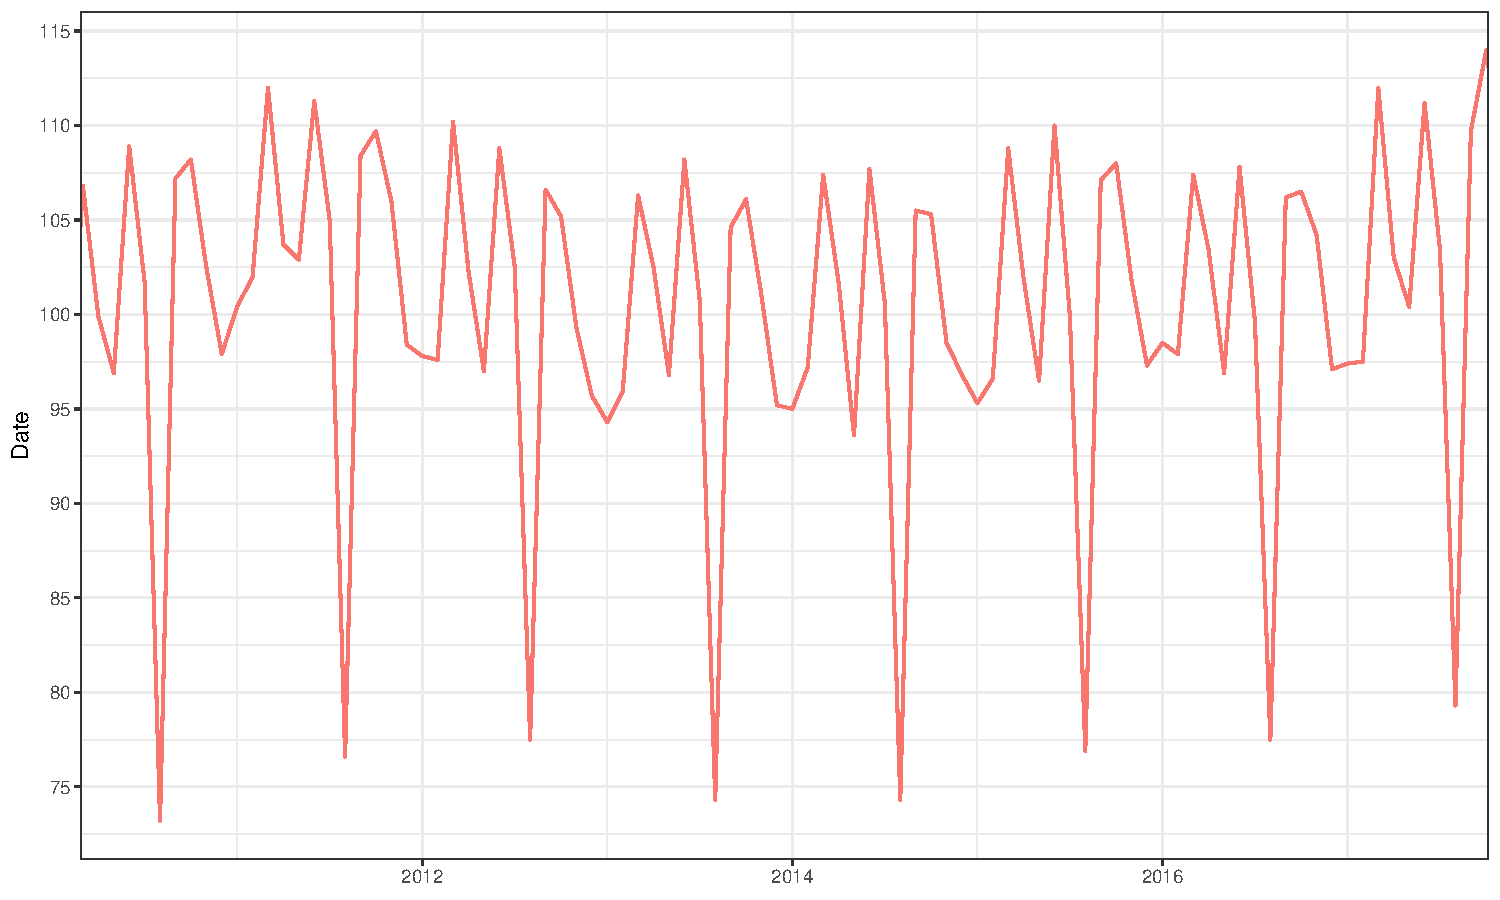
\includegraphics{img/markdown-unnamed-chunk-1-1.pdf}
\caption{Industrial production index in France}
\end{figure}

\end{frame}

\begin{frame}{Introduction to seasonal adjustment (2/3)}
\protect\hypertarget{introduction-to-seasonal-adjustment-23}{}

Purpose of seasonal adjustment:

\begin{itemize}
\tightlist
\item
  Time comparison (outlook, short-term evolution\ldots{})\\
\item
  Spatial comparison
\end{itemize}

\bigskip
\pause

Two leading methods:

\begin{itemize}
\tightlist
\item
  TRAMO/SEATS+ (Bank of Spain)\\
\item
  X-12ARIMA/X-13ARIMA-SEATS (US-Census Bureau).
\end{itemize}

\bigskip
\pause

\(\rightarrow\) proceed in two steps

\end{frame}

\begin{frame}{Introduction to seasonal adjustment (3/3)}
\protect\hypertarget{introduction-to-seasonal-adjustment-33}{}

\vspace{-0.15cm}

\begin{enumerate}
\item
  Pre-adjusting the series of deterministics effects with a RegARIMA
  model
\item
  Decomposition: to extract seasonal component
\end{enumerate}

\centering

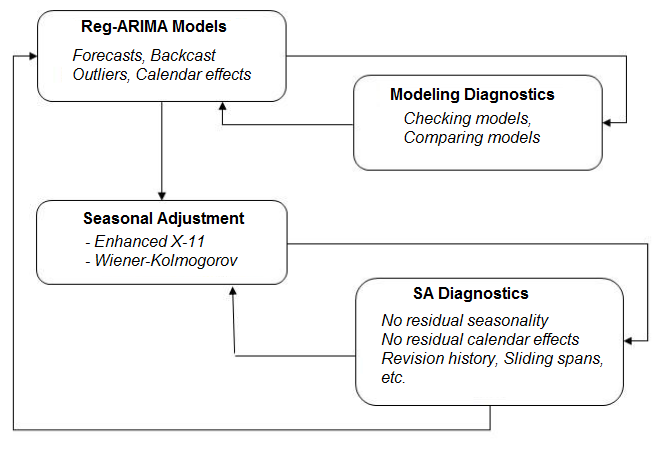
\includegraphics[height=0.75\textheight]{img/sa_2_steps.png}

\end{frame}

\begin{frame}{What's JDemetra+ ?}
\protect\hypertarget{whats-jdemetra}{}


\includegraphics[width=2cm]{img/jdemetra+.jpg} TRAMO/SEATS+ and
X-13ARIMA-SEATS are implemented in JDemetra+

\bigskip

\large\faThumbsUp{} \normalsize Software
\href{https://ec.europa.eu/eurostat/cros/system/files/Jdemetra_\%20release.pdf}{officially
recommended} by Eurostat and the ECB for seasonal and calendar
adjustment of official statistics

\bigskip

\(\rightarrow\) RJDemetra is an \large\faRProject{}
\normalsize interface to JDemetra+ based on the \large\faJava{}
\normalsize libraries of JD+

\end{frame}

\hypertarget{rjdemetra}{%
\section{RJDemetra}\label{rjdemetra}}

\hypertarget{current-status}{%
\subsection{Current status}\label{current-status}}

\begin{frame}{Current status}
\protect\hypertarget{current-status-1}{}

\begin{itemize}
\tightlist
\item
  RegARIMA, TRAMO-SEATS and X-13-ARIMA:

  \begin{itemize}
  \tightlist
  \item
    pre-defined and user-defined specifications\\
  \item
    S3 classes with plot, summary, print methods
  \end{itemize}
\item
  Manipulate JD+ workspaces:

  \begin{itemize}
  \tightlist
  \item
    Import JD+ workspace to get: input raw series or SA model
  \item
    Export R models created via RJDemetra
  \end{itemize}
\item
  Include a dataset: industrial production indices in manufacturing in
  the European Union
\end{itemize}

\end{frame}

\hypertarget{some-examples}{%
\subsection{Some examples}\label{some-examples}}

\begin{frame}[fragile]{RegARIMA examples (1/3)}
\protect\hypertarget{regarima-examples-13}{}

\footnotesize

\begin{Shaded}
\begin{Highlighting}[]
\KeywordTok{library}\NormalTok{(RJDemetra)}
\NormalTok{ipi_fr <-}\StringTok{ }\NormalTok{ipi_c_eu[,}\StringTok{"FR"}\NormalTok{]}
\NormalTok{regarima_model <-}\StringTok{ }\KeywordTok{regarima_def_x13}\NormalTok{(ipi_fr, }\DataTypeTok{spec =} \StringTok{"RG4c"}\NormalTok{)}
\NormalTok{regarima_model}
\end{Highlighting}
\end{Shaded}

\begin{verbatim}
## y = regression model + arima (2, 1, 1, 0, 1, 1)
## Log-transformation: no
## Coefficients:
##           Estimate Std. Error
## Phi(1)      0.3358      0.171
## Phi(2)      0.2060      0.096
## Theta(1)   -0.2450      0.173
## BTheta(1)  -0.5112      0.050
## 
##              Estimate Std. Error
## Easter [1]     -1.133      0.337
## LS (11-2008)   -8.000      1.283
## LS (1-2009)    -7.551      1.283
## LS (5-2008)    -5.069      1.234
## 
## 
## Residual standard error: 1.696 on 323 degrees of freedom
## Log likelihood =  -631, aic =  1280 aicc =  1281, bic(corrected for length) =   1.2
\end{verbatim}

\end{frame}

\begin{frame}[fragile]{RegARIMA examples (2/3)}
\protect\hypertarget{regarima-examples-23}{}

\footnotesize

\begin{Shaded}
\begin{Highlighting}[]
\KeywordTok{summary}\NormalTok{(regarima_model)}
\end{Highlighting}
\end{Shaded}

\begin{verbatim}
## y = regression model + arima (2, 1, 1, 0, 1, 1)
## 
## Model: RegARIMA - X13
## Estimation span: from 1-1990 to 12-2017
## Log-transformation: no
## Regression model: no mean, no trading days effect, no leap year effect, Easter effect, outliers(3)
## 
## Coefficients:
## ARIMA: 
##           Estimate Std. Error  T-stat Pr(>|t|)    
## Phi(1)     0.33579    0.17106   1.963   0.0505 .  
## Phi(2)     0.20600    0.09643   2.136   0.0334 *  
## Theta(1)  -0.24498    0.17272  -1.418   0.1571    
## BTheta(1) -0.51123    0.05004 -10.216   <2e-16 ***
## ---
## Signif. codes:  0 '***' 0.001 '**' 0.01 '*' 0.05 '.' 0.1 ' ' 1
## 
## Regression model: 
##              Estimate Std. Error T-stat Pr(>|t|)    
## Easter [1]    -1.1332     0.3373 -3.359 0.000875 ***
## LS (11-2008)  -7.9997     1.2831 -6.235 1.42e-09 ***
## LS (1-2009)   -7.5508     1.2833 -5.884 1.00e-08 ***
## LS (5-2008)   -5.0692     1.2341 -4.108 5.07e-05 ***
## ---
## Signif. codes:  0 '***' 0.001 '**' 0.01 '*' 0.05 '.' 0.1 ' ' 1
## 
## 
## Residual standard error: 1.696 on 9 degrees of freedom
## Log likelihood =  -631, aic =  1280, aicc =  1281, bic(corrected for length) =   1.2
\end{verbatim}

\end{frame}

\begin{frame}[fragile]{RegARIMA examples (3/3)}
\protect\hypertarget{regarima-examples-33}{}

\begin{Shaded}
\begin{Highlighting}[]
\KeywordTok{layout}\NormalTok{(}\KeywordTok{matrix}\NormalTok{(}\DecValTok{1}\OperatorTok{:}\DecValTok{6}\NormalTok{, }\DecValTok{3}\NormalTok{, }\DecValTok{2}\NormalTok{));}\KeywordTok{plot}\NormalTok{(regarima_model, }\DataTypeTok{ask =} \OtherTok{FALSE}\NormalTok{)}
\end{Highlighting}
\end{Shaded}

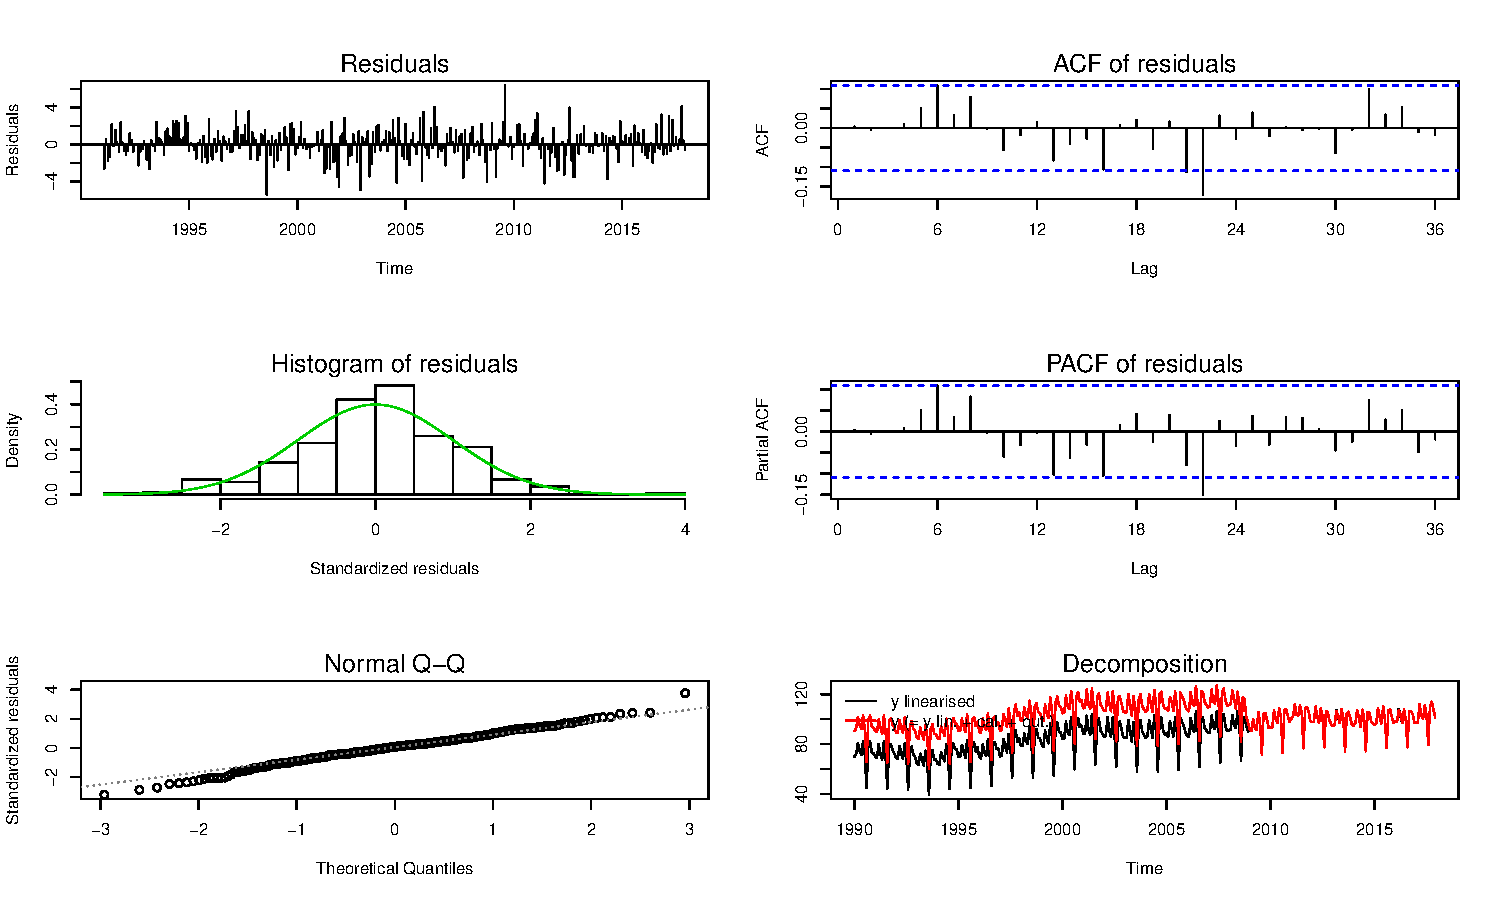
\includegraphics{img/markdown-unnamed-chunk-5-1.pdf}

\end{frame}

\hypertarget{seasonal-adjustment-examples}{%
\subsection{Seasonal adjustment
examples}\label{seasonal-adjustment-examples}}

\begin{frame}[fragile]{Seasonal adjustment examples (1/7)}
\protect\hypertarget{seasonal-adjustment-examples-17}{}

A \texttt{SA} object is a \texttt{list()} of 5 elements:

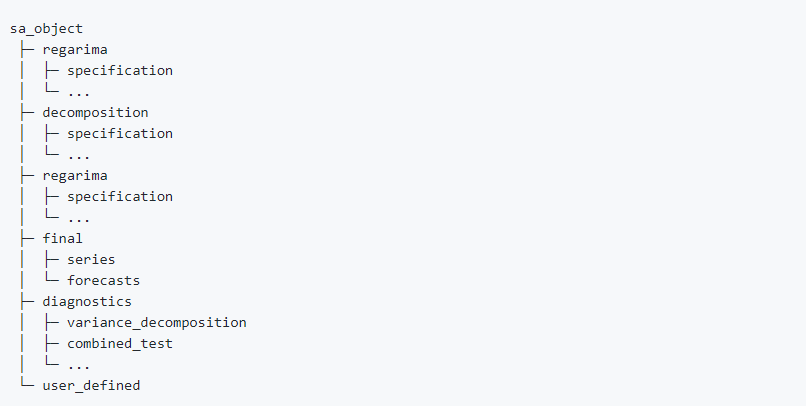
\includegraphics{img/sa_obj_struct.png}

\end{frame}

\begin{frame}[fragile]{Seasonal adjustment examples (2/7)}
\protect\hypertarget{seasonal-adjustment-examples-27}{}

Like in JD+ users can defined their own specification or use a
pre-defined one:

\footnotesize

\begin{Shaded}
\begin{Highlighting}[]
\NormalTok{x13_usr_spec <-}\StringTok{ }\KeywordTok{x13_spec_def}\NormalTok{(}\DataTypeTok{spec =} \KeywordTok{c}\NormalTok{(}\StringTok{"RSA5c"}\NormalTok{),}
                             \DataTypeTok{usrdef.outliersEnabled =} \OtherTok{TRUE}\NormalTok{,}
                             \DataTypeTok{usrdef.outliersType =} \KeywordTok{c}\NormalTok{(}\StringTok{"LS"}\NormalTok{, }\StringTok{"AO"}\NormalTok{),}
                             \DataTypeTok{usrdef.outliersDate =} \KeywordTok{c}\NormalTok{(}\StringTok{"2008-10-01"}\NormalTok{,}
                                                     \StringTok{"2002-01-01"}\NormalTok{),}
                             \DataTypeTok{usrdef.outliersCoef =} \KeywordTok{c}\NormalTok{(}\DecValTok{36}\NormalTok{, }\DecValTok{14}\NormalTok{),}
                             \DataTypeTok{transform.function =} \StringTok{"None"}\NormalTok{)}
\NormalTok{x13_mod <-}\StringTok{ }\KeywordTok{x13}\NormalTok{(ipi_fr, x13_usr_spec)}
\NormalTok{ts_mod <-}\StringTok{ }\KeywordTok{tramoseats_def}\NormalTok{(ipi_fr, }\DataTypeTok{spec =} \StringTok{"RSAfull"}\NormalTok{)}
\end{Highlighting}
\end{Shaded}

\end{frame}

\begin{frame}[fragile]{Seasonal adjustment examples (3/7):
decomposition}
\protect\hypertarget{seasonal-adjustment-examples-37-decomposition}{}

\footnotesize

\begin{Shaded}
\begin{Highlighting}[]
\NormalTok{x13_mod}\OperatorTok{$}\NormalTok{decomposition}
\end{Highlighting}
\end{Shaded}

\begin{verbatim}
##  Monitoring and Quality Assessment Statistics:  
##       M stats
## M(1)    0.055
## M(2)    0.041
## M(3)    0.926
## M(4)    0.621
## M(5)    0.724
## M(6)    0.215
## M(7)    0.074
## M(8)    0.208
## M(9)    0.056
## M(10)   0.158
## M(11)   0.146
## Q       0.297
## Q-M2    0.329
## 
## Final filters: 
## Seasonal filter:  3x5
## Trend filter:  13 terms Henderson moving average
\end{verbatim}

\end{frame}

\begin{frame}[fragile]{Seasonal adjustment examples (4/7):
decomposition}
\protect\hypertarget{seasonal-adjustment-examples-47-decomposition}{}

\footnotesize

\begin{Shaded}
\begin{Highlighting}[]
\NormalTok{ts_mod}\OperatorTok{$}\NormalTok{decomposition}
\end{Highlighting}
\end{Shaded}

\begin{verbatim}
## Model
## AR :  1 + 0.352498 B + 0.133616 B^2 
## D :  1 - B - B^12 + B^13 
## MA :  1 - 0.186819 B - 0.610856 B^12 + 0.114119 B^13 
## 
## 
## SA
## D :  1 - 2.000000 B + B^2 
## MA :  1 - 1.314459 B + 0.340427 B^2 
## Innovation variance:  0.4669153 
## 
## Trend
## D :  1 - 2.000000 B + B^2 
## MA :  1 + 0.040206 B - 0.959794 B^2 
## Innovation variance:  0.04869563 
## 
## Seasonal
## AR :  1 + 0.352498 B + 0.133616 B^2 
## D :  1 + B + B^2 + B^3 + B^4 + B^5 + B^6 + B^7 + B^8 + B^9 + B^10 + B^11 
## MA :  1 + 0.717848 B + 0.460721 B^2 + 0.310085 B^3 + 0.132447 B^4 - 0.049053 B^5 - 0.216655 B^6 - 0.354556 B^7 - 0.445030 B^8 - 0.469587 B^9 - 0.376625 B^10 - 0.166397 B^11 - 0.410618 B^12 - 0.132580 B^13 
## Innovation variance:  0.1601924 
## 
## Irregular
## Innovation variance:  0.2056884
\end{verbatim}

\end{frame}

\begin{frame}[fragile]{Seasonal adjustment examples (5/7)}
\protect\hypertarget{seasonal-adjustment-examples-57}{}

\begin{Shaded}
\begin{Highlighting}[]
\KeywordTok{plot}\NormalTok{(x13_mod}\OperatorTok{$}\NormalTok{decomposition)}
\end{Highlighting}
\end{Shaded}

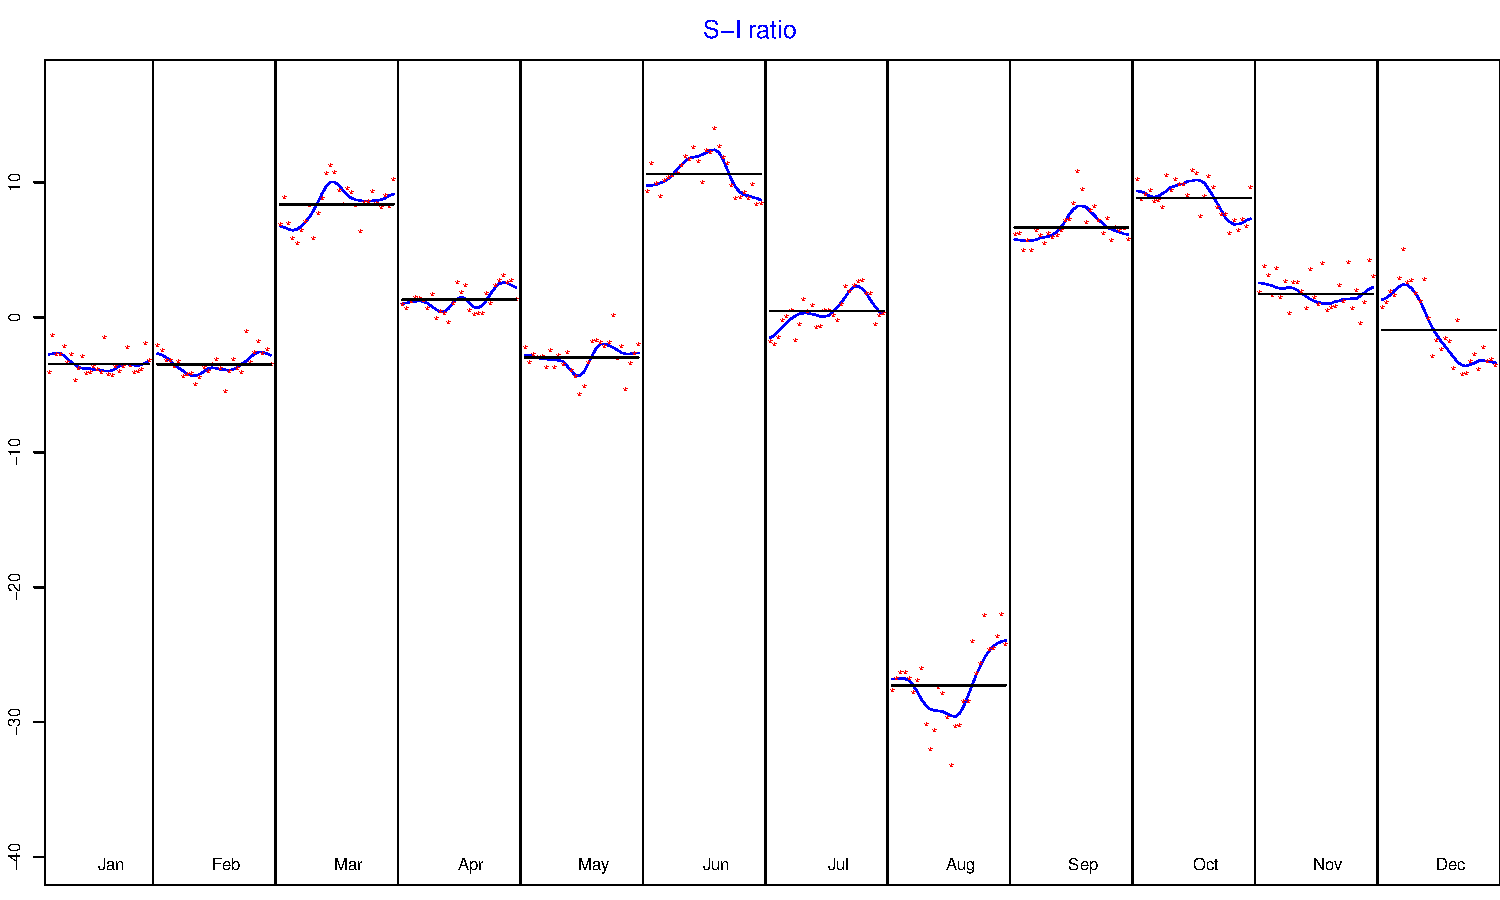
\includegraphics{img/markdown-unnamed-chunk-9-1.pdf}

\end{frame}

\begin{frame}[fragile]{Seasonal adjustment examples (6/7)}
\protect\hypertarget{seasonal-adjustment-examples-67}{}

\footnotesize

\begin{Shaded}
\begin{Highlighting}[]
\NormalTok{x13_mod}\OperatorTok{$}\NormalTok{final}
\end{Highlighting}
\end{Shaded}

\begin{verbatim}
## Last observed values
##              y       sa        t           s             i
## Jan 2017  97.4 100.6172 100.6174  -3.2172329 -0.0001992082
## Feb 2017  97.5 100.3127 101.0283  -2.8126932 -0.7155966863
## Mar 2017 112.0 102.5469 101.4894   9.4530696  1.0575376567
## Apr 2017 103.0 101.0897 101.9282   1.9103111 -0.8385432983
## May 2017 100.4 103.0319 102.3136  -2.6318733  0.7182480125
## Jun 2017 111.2 102.4926 102.6921   8.7074293 -0.1994894034
## Jul 2017 103.4 103.1596 103.0816   0.2404277  0.0779236963
## Aug 2017  79.3 103.2483 103.5055 -23.9483256 -0.2572170473
## Sep 2017 109.7 103.5536 103.9555   6.1464361 -0.4019376040
## Oct 2017 114.0 106.6886 104.3955   7.3113786  2.2931579296
## Nov 2017 107.7 105.4631 104.7505   2.2369236  0.7125546908
## Dec 2017 101.4 104.7490 105.0214  -3.3490189 -0.2723590878
## 
## Forecasts:
##                y_f     sa_f      t_f         s_f          i_f
## Jan 2018 101.96630 105.0963 105.1795  -3.1299775 -0.083200162
## Feb 2018 102.23632 105.1464 105.2838  -2.9100563 -0.137428535
## Mar 2018 113.85794 105.5026 105.3966   8.3553336  0.105971540
## Apr 2018 108.47477 105.4896 105.5573   2.9851827 -0.067754048
## May 2018 103.22164 105.7963 105.7844  -2.5746309  0.011859024
## Jun 2018 114.64042 106.0073 106.0629   8.6331483 -0.055612674
## Jul 2018 106.53519 106.3942 106.3666   0.1410119  0.027594337
## Aug 2018  82.77073 106.6890 106.6849 -23.9182264  0.004061745
## Sep 2018 112.79551 106.7018 106.9859   6.0936895 -0.284129714
## Oct 2018 115.13202 107.7516 107.2471   7.3803800  0.504589345
## Nov 2018 109.87965 107.5136 107.4572   2.3660966  0.056314698
## Dec 2018 103.97193 107.3744 107.6093  -3.4024325 -0.234923742
\end{verbatim}

\end{frame}

\begin{frame}[fragile]{Seasonal adjustment examples (7/7)}
\protect\hypertarget{seasonal-adjustment-examples-77}{}

\begin{Shaded}
\begin{Highlighting}[]
\KeywordTok{plot}\NormalTok{(x13_mod}\OperatorTok{$}\NormalTok{final, }\DataTypeTok{first_date =} \DecValTok{2012}\NormalTok{, }\DataTypeTok{type_chart =} \StringTok{"sa-trend"}\NormalTok{)}
\end{Highlighting}
\end{Shaded}

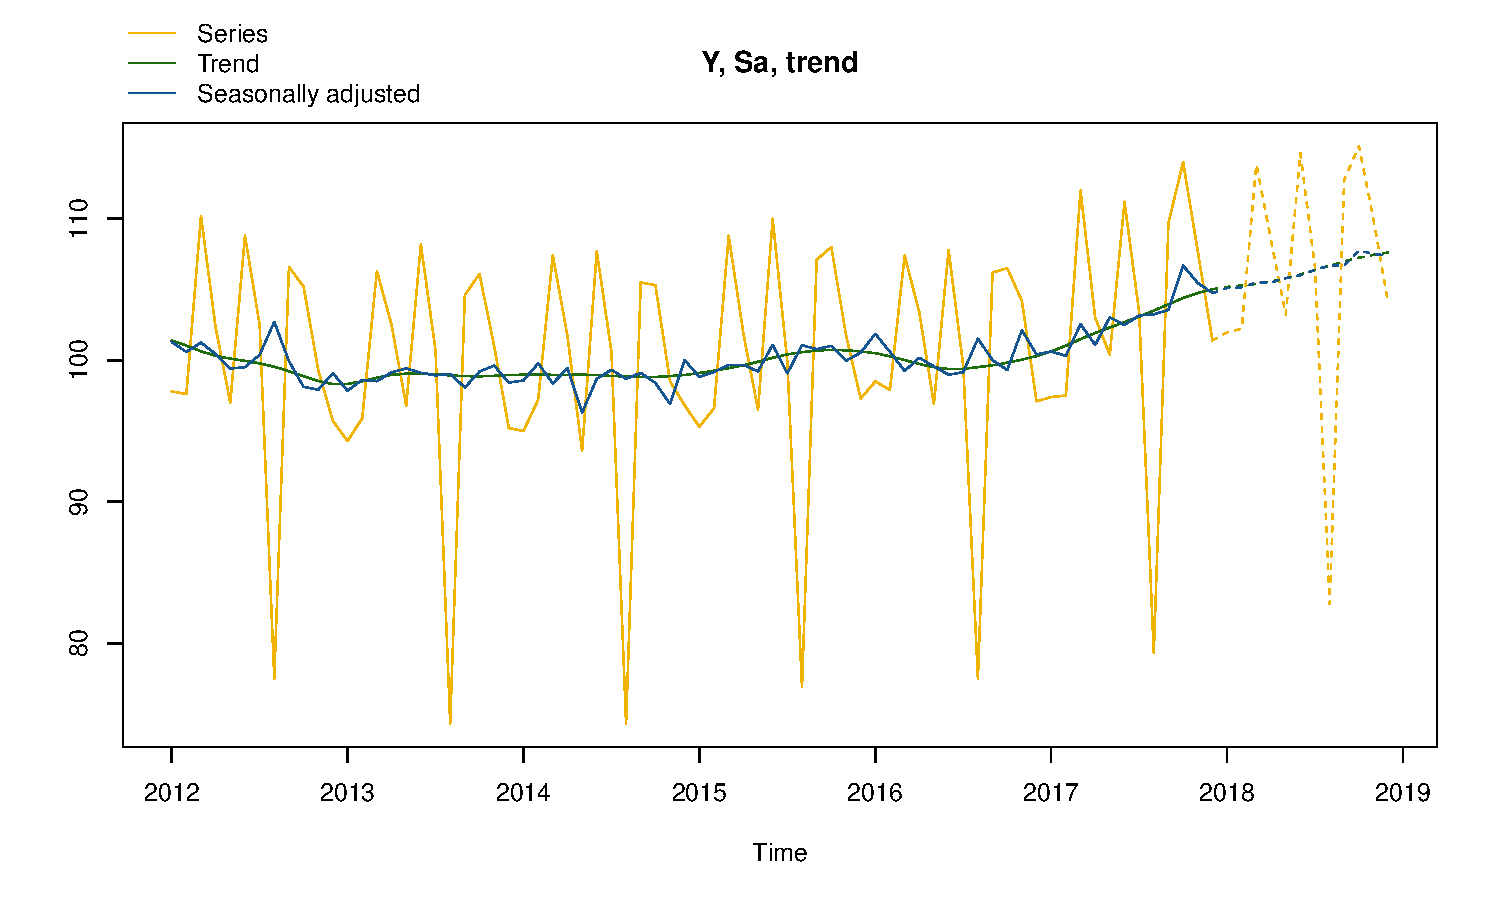
\includegraphics{img/markdown-unnamed-chunk-11-1.pdf}

\end{frame}

\begin{frame}[fragile]{Seasonal adjustment examples (8/7)}
\protect\hypertarget{seasonal-adjustment-examples-87}{}

\footnotesize

\begin{Shaded}
\begin{Highlighting}[]
\NormalTok{x13_mod}\OperatorTok{$}\NormalTok{diagnostics}
\end{Highlighting}
\end{Shaded}

\begin{verbatim}
##  Relative contribution of the components to the stationary
##  portion of the variance in the original series,
##  after the removal of the long term trend 
##  Trend computed by Hodrick-Prescott filter (cycle length = 8.0 years)
##            Component
##  Cycle         1.557
##  Seasonal     39.219
##  Irregular     0.362
##  TD & Hol.     0.018
##  Others       61.971
##  Total       103.128
## 
##  Combined test in the entire series 
##  Non parametric tests for stable seasonality
##                                                           P.value
##    Kruskall-Wallis test                                      0.000
##    Test for the presence of seasonality assuming stability   0.000
##    Evolutive seasonality test                                0.032
##  
##  Identifiable seasonality present
## 
##  Residual seasonality tests 
##                                       P.value
##  qs test on sa                          1.000
##  qs test on i                           1.000
##  f-test on sa (seasonal dummies)        0.997
##  f-test on i (seasonal dummies)         0.965
##  Residual seasonality (entire series)   0.993
##  Residual seasonality (last 3 years)    0.922
##  f-test on sa (td)                      0.001
##  f-test on i (td)                       0.006
\end{verbatim}

\end{frame}

\hypertarget{manipulate-workspaces}{%
\subsection{Manipulate workspaces}\label{manipulate-workspaces}}

\begin{frame}[fragile]{Export a workspace}
\protect\hypertarget{export-a-workspace}{}

\footnotesize

\begin{Shaded}
\begin{Highlighting}[]
\NormalTok{wk <-}\StringTok{ }\KeywordTok{new_workspace}\NormalTok{()}
\KeywordTok{new_multiprocessing}\NormalTok{(wk, }\DataTypeTok{name =} \StringTok{"MP-1"}\NormalTok{)}
\KeywordTok{add_sa_item}\NormalTok{(wk, }\DataTypeTok{multiprocessing =} \StringTok{"MP-1"}\NormalTok{,}
            \DataTypeTok{sa_obj =}\NormalTok{ x13_mod, }\DataTypeTok{name =}  \StringTok{"SA with X13 model 1 "}\NormalTok{)}
\KeywordTok{add_sa_item}\NormalTok{(wk, }\DataTypeTok{multiprocessing =}  \StringTok{"MP-1"}\NormalTok{,}
            \DataTypeTok{sa_obj =}\NormalTok{ ts_mod, }\DataTypeTok{name =} \StringTok{"SA with TramoSeats model 1"}\NormalTok{)}
\KeywordTok{save_workspace}\NormalTok{(wk, }\StringTok{"workspace.xml"}\NormalTok{)}
\end{Highlighting}
\end{Shaded}

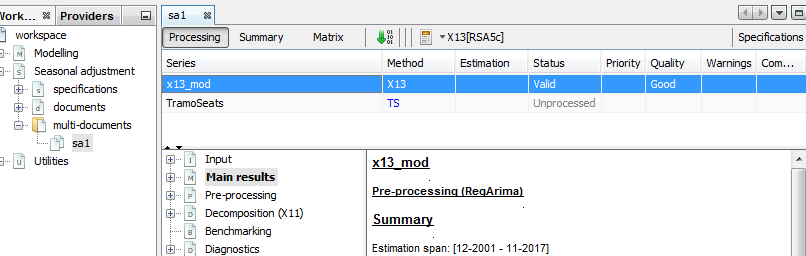
\includegraphics{img/workspace.png}

\end{frame}

\begin{frame}[fragile]{Import a workspace (1/3)}
\protect\hypertarget{import-a-workspace-13}{}

\footnotesize

\begin{Shaded}
\begin{Highlighting}[]
\NormalTok{wk <-}\StringTok{ }\KeywordTok{load_workspace}\NormalTok{(}\StringTok{"workspace.xml"}\NormalTok{)}
\KeywordTok{get_ts}\NormalTok{(wk)}
\end{Highlighting}
\end{Shaded}

\begin{verbatim}
## $`MP-1`
## $`MP-1`$`SA with X13 model 1 `
##        Jan   Feb   Mar   Apr   May   Jun   Jul   Aug   Sep   Oct   Nov
## 1990  90.5  92.6 101.9  95.2  92.1 103.3  91.8  65.5  99.0 102.8  94.3
## 1991  90.9  89.6  99.9  93.3  88.3 103.0  89.7  65.1  98.2 100.8  95.8
## 1992  89.4  89.0  99.5  93.0  89.1 101.3  89.4  64.1  94.9  98.6  92.2
## 1993  85.3  84.3  93.2  87.8  83.5  95.4  86.2  60.1  92.1  95.8  88.1
## 1994  84.9  84.0  94.1  90.1  86.8 100.4  90.8  64.5  96.8 101.0  96.6
## 1995  90.4  90.5 100.4  94.5  89.7 103.7  93.8  65.5  99.7 101.8  94.6
## 1996  90.3  88.8 100.7  93.8  91.2 104.4  92.3  67.2 100.2 102.3  96.9
## 1997  90.5  91.6 104.0  99.7  93.9 108.8  98.2  73.4 105.8 111.8 102.4
## 1998  99.2  99.0 109.4 103.0 100.7 114.8 104.9  73.3 109.6 112.7 105.9
## 1999 100.5  98.6 111.8 104.3 101.3 117.4 106.6  74.9 113.4 118.2 110.9
## 2000 104.8 104.9 118.9 110.2 108.0 122.5 111.8  80.5 117.5 121.7 114.3
## 2001 108.8 109.2 123.7 111.8 108.4 124.7 111.1  84.2 117.8 121.0 111.6
## 2002 106.6 107.0 121.4 112.8 106.4 122.2 109.7  82.3 117.1 118.7 113.0
## 2003 105.4 105.7 120.1 111.1 102.8 118.3 108.8  78.7 115.9 119.9 110.8
## 2004 105.8 107.0 120.0 112.1 105.8 123.6 112.0  78.4 120.0 122.0 112.0
## 2005 109.1 106.7 117.9 113.5 106.8 122.3 110.3  80.0 121.4 118.4 115.2
## 2006 107.3 106.3 121.9 112.5 110.8 126.7 112.5  82.5 122.2 121.9 113.7
## 2007 109.5 110.0 123.8 114.2 112.6 127.0 115.2  85.7 121.2 124.7 115.2
## 2008 111.4 112.2 123.0 116.8 108.4 122.1 112.6  81.9 117.3 116.3 102.4
## 2009  91.7  90.4 100.1  93.2  91.4 105.5  96.8  71.6 104.5 104.8  99.3
## 2010  93.7  93.5 106.8  99.9  96.9 108.9 101.7  73.2 107.2 108.2 102.5
## 2011 100.4 102.0 112.0 103.7 102.9 111.3 105.0  76.6 108.4 109.7 106.0
## 2012  97.8  97.6 110.2 102.3  97.0 108.8 102.5  77.5 106.6 105.2  99.3
## 2013  94.3  95.9 106.3 102.5  96.8 108.2 100.7  74.3 104.6 106.1 101.0
## 2014  95.0  97.2 107.4 101.7  93.6 107.7 100.6  74.3 105.5 105.3  98.5
## 2015  95.3  96.6 108.8 101.9  96.5 110.0  99.9  76.9 107.1 108.0 101.8
## 2016  98.5  97.9 107.4 103.4  96.9 107.8  99.6  77.5 106.2 106.5 104.2
## 2017  97.4  97.5 112.0 103.0 100.4 111.2 103.4  79.3 109.7 114.0 107.7
##        Dec
## 1990  93.1
## 1991  93.2
## 1992  90.5
## 1993  88.3
## 1994  96.3
## 1995  98.1
## 1996  97.2
## 1997 105.4
## 1998 105.1
## 1999 109.8
## 2000 115.5
## 2001 109.2
## 2002 106.4
## 2003 107.9
## 2004 108.4
## 2005 109.8
## 2006 111.7
## 2007 111.0
## 2008  97.8
## 2009  92.9
## 2010  97.9
## 2011  98.4
## 2012  95.7
## 2013  95.2
## 2014  96.8
## 2015  97.3
## 2016  97.1
## 2017 101.4
## 
## $`MP-1`$`SA with TramoSeats model 1`
##        Jan   Feb   Mar   Apr   May   Jun   Jul   Aug   Sep   Oct   Nov
## 1990  90.5  92.6 101.9  95.2  92.1 103.3  91.8  65.5  99.0 102.8  94.3
## 1991  90.9  89.6  99.9  93.3  88.3 103.0  89.7  65.1  98.2 100.8  95.8
## 1992  89.4  89.0  99.5  93.0  89.1 101.3  89.4  64.1  94.9  98.6  92.2
## 1993  85.3  84.3  93.2  87.8  83.5  95.4  86.2  60.1  92.1  95.8  88.1
## 1994  84.9  84.0  94.1  90.1  86.8 100.4  90.8  64.5  96.8 101.0  96.6
## 1995  90.4  90.5 100.4  94.5  89.7 103.7  93.8  65.5  99.7 101.8  94.6
## 1996  90.3  88.8 100.7  93.8  91.2 104.4  92.3  67.2 100.2 102.3  96.9
## 1997  90.5  91.6 104.0  99.7  93.9 108.8  98.2  73.4 105.8 111.8 102.4
## 1998  99.2  99.0 109.4 103.0 100.7 114.8 104.9  73.3 109.6 112.7 105.9
## 1999 100.5  98.6 111.8 104.3 101.3 117.4 106.6  74.9 113.4 118.2 110.9
## 2000 104.8 104.9 118.9 110.2 108.0 122.5 111.8  80.5 117.5 121.7 114.3
## 2001 108.8 109.2 123.7 111.8 108.4 124.7 111.1  84.2 117.8 121.0 111.6
## 2002 106.6 107.0 121.4 112.8 106.4 122.2 109.7  82.3 117.1 118.7 113.0
## 2003 105.4 105.7 120.1 111.1 102.8 118.3 108.8  78.7 115.9 119.9 110.8
## 2004 105.8 107.0 120.0 112.1 105.8 123.6 112.0  78.4 120.0 122.0 112.0
## 2005 109.1 106.7 117.9 113.5 106.8 122.3 110.3  80.0 121.4 118.4 115.2
## 2006 107.3 106.3 121.9 112.5 110.8 126.7 112.5  82.5 122.2 121.9 113.7
## 2007 109.5 110.0 123.8 114.2 112.6 127.0 115.2  85.7 121.2 124.7 115.2
## 2008 111.4 112.2 123.0 116.8 108.4 122.1 112.6  81.9 117.3 116.3 102.4
## 2009  91.7  90.4 100.1  93.2  91.4 105.5  96.8  71.6 104.5 104.8  99.3
## 2010  93.7  93.5 106.8  99.9  96.9 108.9 101.7  73.2 107.2 108.2 102.5
## 2011 100.4 102.0 112.0 103.7 102.9 111.3 105.0  76.6 108.4 109.7 106.0
## 2012  97.8  97.6 110.2 102.3  97.0 108.8 102.5  77.5 106.6 105.2  99.3
## 2013  94.3  95.9 106.3 102.5  96.8 108.2 100.7  74.3 104.6 106.1 101.0
## 2014  95.0  97.2 107.4 101.7  93.6 107.7 100.6  74.3 105.5 105.3  98.5
## 2015  95.3  96.6 108.8 101.9  96.5 110.0  99.9  76.9 107.1 108.0 101.8
## 2016  98.5  97.9 107.4 103.4  96.9 107.8  99.6  77.5 106.2 106.5 104.2
## 2017  97.4  97.5 112.0 103.0 100.4 111.2 103.4  79.3 109.7 114.0 107.7
##        Dec
## 1990  93.1
## 1991  93.2
## 1992  90.5
## 1993  88.3
## 1994  96.3
## 1995  98.1
## 1996  97.2
## 1997 105.4
## 1998 105.1
## 1999 109.8
## 2000 115.5
## 2001 109.2
## 2002 106.4
## 2003 107.9
## 2004 108.4
## 2005 109.8
## 2006 111.7
## 2007 111.0
## 2008  97.8
## 2009  92.9
## 2010  97.9
## 2011  98.4
## 2012  95.7
## 2013  95.2
## 2014  96.8
## 2015  97.3
## 2016  97.1
## 2017 101.4
\end{verbatim}

\end{frame}

\begin{frame}[fragile]{Import a workspace (2/3)}
\protect\hypertarget{import-a-workspace-23}{}

\footnotesize

\begin{Shaded}
\begin{Highlighting}[]
\KeywordTok{compute}\NormalTok{(wk) }\CommentTok{# Important to get the Sa model}
\NormalTok{models <-}\StringTok{ }\KeywordTok{get_model}\NormalTok{(wk) }\CommentTok{# A progress bar is printed by default}
\end{Highlighting}
\end{Shaded}

\begin{verbatim}
## Multiprocessing 1 on 1:
## 
  |                                                                       
  |                                                                 |   0%
  |                                                                       
  |================================                                 |  50%
  |                                                                       
  |=================================================================| 100%
\end{verbatim}

\begin{Shaded}
\begin{Highlighting}[]
\CommentTok{# To extract only one model}
\NormalTok{mp <-}\StringTok{ }\KeywordTok{get_object}\NormalTok{(wk, }\DecValTok{1}\NormalTok{)}
\KeywordTok{count}\NormalTok{(mp)}
\end{Highlighting}
\end{Shaded}

\begin{verbatim}
## [1] 2
\end{verbatim}

\begin{Shaded}
\begin{Highlighting}[]
\NormalTok{sa2 <-}\StringTok{ }\KeywordTok{get_object}\NormalTok{(mp,}\DecValTok{2}\NormalTok{)}
\KeywordTok{get_name}\NormalTok{(sa2)}
\end{Highlighting}
\end{Shaded}

\begin{verbatim}
## [1] "SA with TramoSeats model 1"
\end{verbatim}

\begin{Shaded}
\begin{Highlighting}[]
\NormalTok{mod <-}\StringTok{ }\KeywordTok{get_model}\NormalTok{(wk, sa2)}
\end{Highlighting}
\end{Shaded}

\begin{verbatim}
## Multiprocessing 1 on 1:
## 
  |                                                                       
  |                                                                 |   0%
  |                                                                       
  |================================                                 |  50%
  |                                                                       
  |=================================================================| 100%
\end{verbatim}

\end{frame}

\begin{frame}{Import a workspace (2/3)}
\protect\hypertarget{import-a-workspace-23-1}{}

\animategraphics[loop, autoplay, width=\linewidth]{3}{img/gif/import_model/}{1}{97}

\end{frame}

\hypertarget{installation-and-future-development}{%
\subsection{Installation and future
development}\label{installation-and-future-development}}

\begin{frame}[fragile]{How to install the package?}
\protect\hypertarget{how-to-install-the-package}{}

The package is available on GitHub:
\url{https://github.com/jdemetra/rjdemetra}

It has also it's own website:
\url{https://jdemetra.github.io/rjdemetra/}

It package can be installed from CRAN:

\begin{Shaded}
\begin{Highlighting}[]
\KeywordTok{install.packages}\NormalTok{(}\StringTok{"RJDemetra"}\NormalTok{)}
\end{Highlighting}
\end{Shaded}

Or from github (development version):

\begin{Shaded}
\begin{Highlighting}[]
\NormalTok{devtools}\OperatorTok{::}\KeywordTok{install_github}\NormalTok{(}\StringTok{"jdemetra/rjdemetra"}\NormalTok{)}
\end{Highlighting}
\end{Shaded}

\bcinfo To install it you need Java8: in case you don't, install a
portable version of Java8 and set the \texttt{JAVA\_HOME} path.

\end{frame}

\hypertarget{future-developments}{%
\subsection{Future developments}\label{future-developments}}

\begin{frame}{What's next? \bcpanchant (1/2)}
\protect\hypertarget{whats-next-12}{}

Documentation:

\begin{itemize}
\item
  Vignette/article for the Journal of Statistical Software
\item
  Guide to install the package with portable version of Java (when you
  don't have administrator rights)
\item
  Cheat sheet
\end{itemize}

\end{frame}

\begin{frame}{What's next? \bcpanchant (2/2)}
\protect\hypertarget{whats-next-22}{}

Package:

\begin{itemize}
\item
  Get only the Java object of a SA (to reduce computation/customize the
  output)
\item
  Possibility to used user-defined calendar regressors (currently: only
  user-defined regressors)
\item
  Function to ``refresh'' the model (JD+ 3.0.0)
\end{itemize}

\end{frame}

\hypertarget{how-to-use-jdemetra-to-improve-production-of-sa-series}{%
\section{How to use JDemetra+ to improve production of SA
series?}\label{how-to-use-jdemetra-to-improve-production-of-sa-series}}

\begin{frame}{Examples of current use of RJDemetra}
\protect\hypertarget{examples-of-current-use-of-rjdemetra}{}

\begin{itemize}
\tightlist
\item
  rjdqa (experimental, no documentation): package to help quality
  assessment (dashboard and quality report matrix)
\end{itemize}

\faGithub{} \url{https://github.com/AQLT/rjdqa}

\begin{itemize}
\tightlist
\item
  persephone: enable easy processing during production of SA series
  (interactive plots, dashboards\ldots{})
\end{itemize}

\faGithub{} \url{https://github.com/statistikat/persephone}

\begin{itemize}
\item
  Non explore topics: direct vs indirect adjustment (persephone),
  analyse of revisions, etc.
\item
  Carry out studies on SA: Ladiray D., Quartier-la-Tente A.,
  ``(In)Stability of Reg-ARIMA Models for Seasonal Adjustment''
  \(\rightarrow\) STS05 in room MANS
\end{itemize}

\end{frame}

\begin{frame}{Thank you for your attention}
\protect\hypertarget{thank-you-for-your-attention}{}

\vspace{-0.2cm}

\begin{columns}
\begin{column}{0.4\textwidth}
\begin{center}

\includegraphics[width=4cm]{img/rjdemetra_logo.png}
\end{center}
\end{column}
\begin{column}{0.5\textwidth} 
\href{https://github.com/jdemetra/rjdemetra}{\faGithub{} jdemetra/rjdemetra}  

\href{https://twitter.com/JDemetraPlus}{\faTwitter{} @JdemetraPlus}

Other works and packages around JD+:  
\href{https://github.com/nbbrd}{\faGithub{} nbbrd}  
\end{column}
\end{columns}

\vfill

Contact:\\
Alain Quartier-la-Tente\\
\href{mailto:alain.quartier-la-tente@insee.fr}{\faEnvelope{} alain.quartier-la-tente@insee.fr}\\
\href{https://twitter.com/AQLT}{\faTwitter{} @AQLT}\\
\href{https://github.com/AQLT}{\faGithub{} AQLT}

\end{frame}

\end{document}
